\section{Introduction}
\label{sec:intro}
\begin{figure}[t!]
    \centering 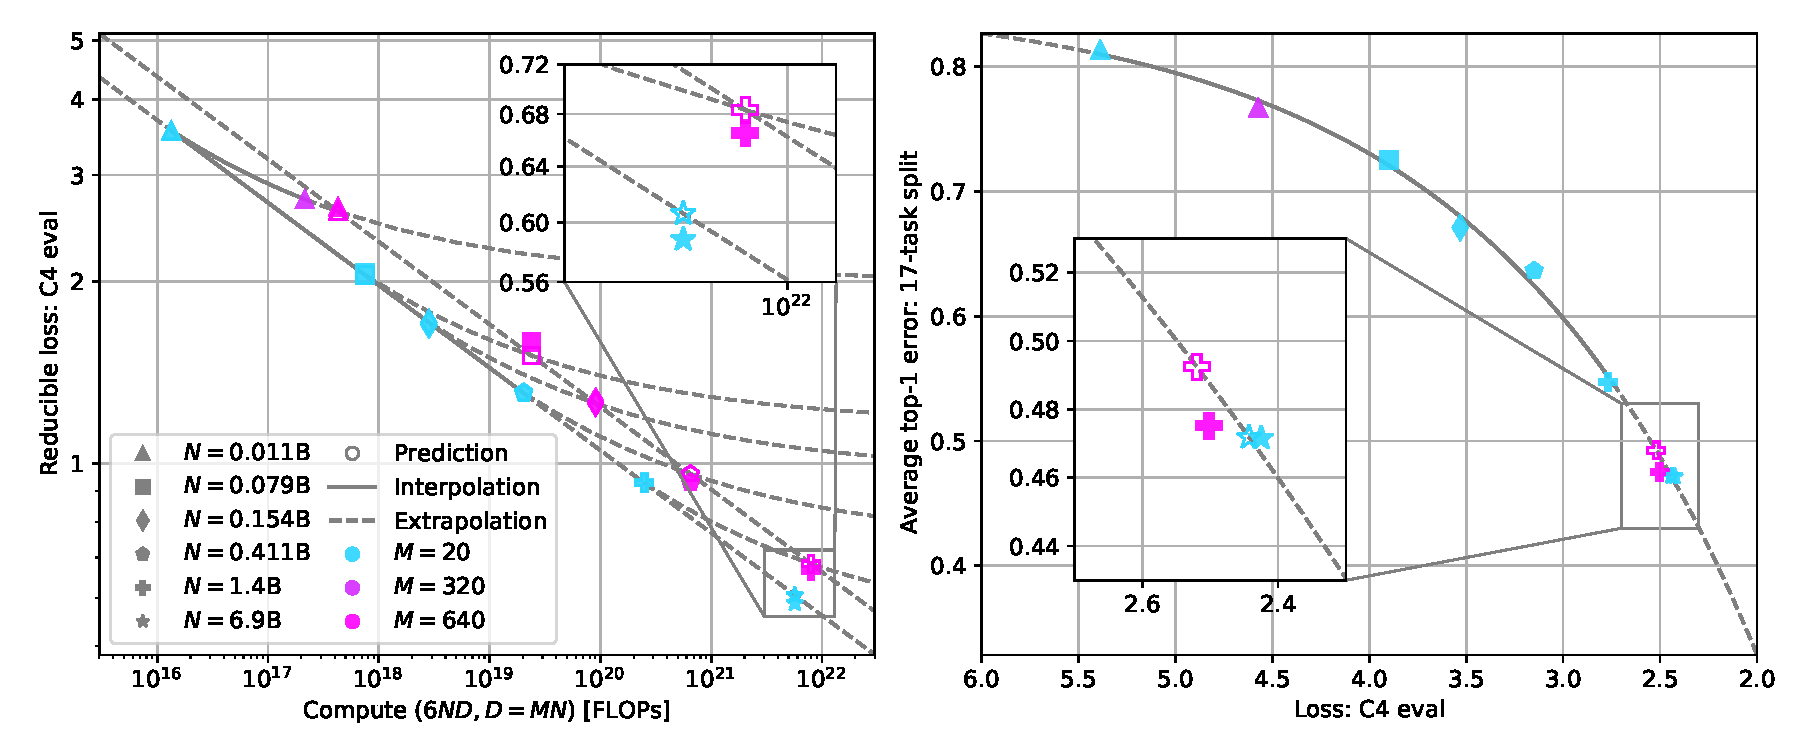
\includegraphics[width=\linewidth]{figs/figure1_rpj_c4_val.pdf}
    \caption{
    \textbf{Reliable scaling with over-training and on downstream error prediction.}
    \emph{(left)}
    We fit a scaling law for model validation loss, parameterized by (i) a token multiplier $M = N/D$, which is the ratio of training tokens $D$ to parameters $N$ and (ii) the compute $C$ in FLOPs used to train a model, approximated by $C=6ND$.
    Larger values of $M$ specify more over-training.
    We are able to extrapolate, in both $N$ and $M$, the validation performance of models requiring more than $300\times$ the training compute used to construct the scaling law.
    \emph{(right)}
    We also fit a scaling law to predict average downstream top-1 error as a function of validation loss.
    We find that fitting scaling laws for downstream error benefits from using more expensive models when compared to fitting for loss prediction.
    We predict the average error over 17 downstream tasks for models trained with over 20$\times$ the compute.
    For this figure, we train all models on RedPajama~\cite{rpj}.
    }
    \label{fig:fig1}
    \vspace*{-3mm}
\end{figure}

Training large language models is expensive.
Furthermore, training high-quality models requires a complex recipe of algorithmic techniques and training data.
To reduce the cost of finding successful training recipes, researchers first evaluate ideas with small experiments and then extrapolate their efficacy to larger model and data regimes via scaling laws.
With reliable extrapolation, it is possible to quickly iterate at small scale and still pick the method that will perform best for the final large training run.
Indeed, this workflow has become commonplace for training state-of-the-art language models like Chinchilla~70B~\cite{chinchilla}, PaLM~540B~\cite{Chowdhery2022PaLMSL}, GPT-4~\cite{gpt4}, and many others.

Despite their importance for model development, published scaling laws differ from the goals of training state-of-the-art models in important ways.
For instance, scaling studies usually focus on the compute-optimal training regime (``Chinchilla optimality''~\cite{chinchilla}), where model and dataset size are set to yield minimum loss for a given compute budget. However, this setting ignores inference costs. As larger models are more expensive at inference, it is now common practice to over-train smaller models~\cite{llama}. Another potential mismatch is that most scaling laws quantify model performance by perplexity in next-token prediction instead of accuracy on widely used benchmark datasets. However, practitioners usually turn to benchmark performance, not loss, to compare models.

In this paper, we conduct an extensive set of experiments to address both scaling in the over-trained regime and benchmark performance prediction.

Motivated by the practice of training beyond compute-optimality, we first investigate whether scaling follows reliable trends in the over-trained regime.
We notice, as implied by~\citet{chinchilla}, for a set of models of different sizes trained with a constant ratio of tokens to parameters, models' reducible loss $L'$~\cite{og_scaling,chinchilla} follows a power law ($L' = \lambda \cdot C^{-\eta}$) in the amount of training compute $C$.
We find that as one increases the ratio of tokens to parameters, corresponding to more over-training, the scaling exponent $\eta$ remains about the same, while the scalar $\lambda$ changes. We explain our observations by reparameterizing existing scaling laws in relation to the amount of over-training.

To establish empirically that scaling \emph{extrapolates} in the over-trained regime, we further experiment with a testbed of 104 models, trained from scratch on three different datasets: C4~\cite{c4,c4_ai2}, RedPajama~\cite{rpj}, and RefinedWeb~\cite{refinedweb}. 
We find that scaling laws fit to small models can accurately predict the performance of larger models that undergo more over-training.
Figure~\ref{fig:fig1} \emph{(left)} illustrates our main over-training result, where we invest $2.4e19$ FLOPs to extrapolate the C4 validation performance of a 1.4B parameter model trained on 900B tokens, which requires $300\times$ more compute to train.

In addition to over-training, we also investigate if scaling laws can predict the performance of a model on downstream tasks.
We establish a power law relationship between language modeling perplexity and the average top-1 error on a suite of downstream tasks.
While it can be difficult to predict the error on individual tasks, we find it possible to predict aggregate performance from a model's perplexity among models trained on the same training data.
Figure~\ref{fig:fig1}~\emph{(right)} presents our main downstream error prediction result, where we invest $2.7e20$ FLOPs to predict the average top-1 error over a set of downstream tasks to within 1 percentage point for a 6.9B compute-optimal model, which requires $20\times$ more compute to train.

Our results suggest that the proposed scaling laws are promising to derisk (i) the effects of over-training models and (ii) the downstream performance of scaling up training recipes.
To facilitate further research on reliable scaling, we provide all results of our experiments at \url{https://github.com/mlfoundations/scaling}.